\section{Introduction} 
<<<<<<< HEAD

Rapidly exploring random tree (RRT) is a path planning algorithm which explores a space by building a tree of random possible moves. 
Each branch is built by extending in a random direction.
The extend distance is called \(\epsilon\).
=======
Rapidly exploring random tree (RRT) is a path planning algorithm which builds a tree of random possible moves. 
Each branch is build by extending in a random direction.
This expansion distance called \(\epsilon\) \citep{pathplanning}.
>>>>>>> 13b64743a88173673163d9c8af9a4d300a4eddec

The bidirectional RRT is a method which builds two trees, one from the goal position and one from the start position. 
When the entire space is explored, a path can be found as a series of steps.

The Balanced Bidirectional RRT is a method which ensures that both trees are of the same size. 
This method is good for getting out of traps where there is plenty of space in the wrong directions.

A KukaKr16 robot is given the task of picking up a bottle from a crate and placing it on a table.
The space is confined by a wall and truck so the robot has to spin around itself in order to reach the goal.
The simulated setup can be seen in figure \ref{fig:worckcell_bottle_picked}.

\begin{figure}[H]
 \centering
 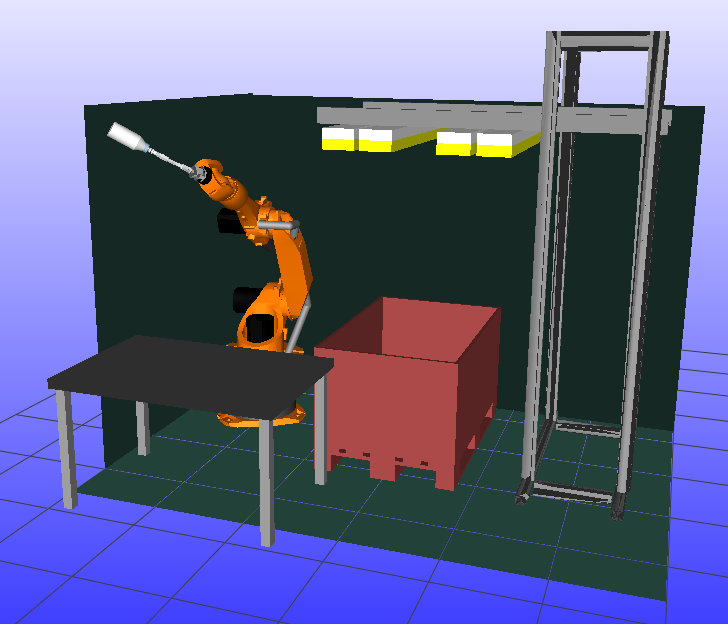
\includegraphics[width=\figsize]{graphics/robworkpic}
 \caption{RobWork simulation workcell with KukaKr16 robot.
 The RRT algorithms are applied to the problem of moving the bottle
 in a collision-free path from the red box to the table.}
 \label{fig:worckcell_bottle_picked}
\end{figure}

The RRT planners takes a parameter, \(\epsilon\), which defines the aggressiveness of the algorithm.
To evaluate the performance of the algorithm, the path length, \(d_J\), is calculated.
Since the space is explored in random directions, the path length will not be the same after every trial.
The hypothesis is the \(\epsilon\) is correlated with the path length and thus there is an optimal \(\epsilon\) for the given configuration.

For each algorithm, the optimal value of this parameter is found with respect to the total joint space distance traveled by the simulated serial robot.
The hypothesis is that the Balanced Bidirectional RRT will perform better in a confined space. % if we want to reject